% =============================================================================
% PART B - MODULE 43: PAYMENTS, STRIPE ESCROW & CONNECT PAYOUTS (UC-43.01 - 43.13)
% In Charge: Vo Nhut Tin (CE180619)
% =============================================================================

\newpage
\subsection{Module 43: Payments, Stripe Escrow \& Connect Payouts}

The Payments \& Stripe Escrow module manages PCI-compliant card storage, Stripe Connect Express payouts onboarding for Freelancers, contract signature escrow hold pre-authorizations, milestone escrow deposits (Checkout and saved-card 1-click funding), automated 95\% milestone releases, and full transaction ledger tracking.

% -----------------------------------------------------------------------------
\subsubsection{M43.01 -- Connect Stripe Payout Account (UC-43.01)}

\begin{itemize}[leftmargin=1.5em,itemsep=2pt]
  \item \textbf{Screen Name \& Route Path:} Billing \& Payments Dashboard -- \texttt{/freelancer/\allowbreak{}payments}.
  \item \textbf{Target Actor:} Freelancer.
  \item \Needspace{6\baselineskip}\textbf{Before You Begin:} Signed in as Freelancer with an active account.
\end{itemize}
\begin{figure}[H]\centering
  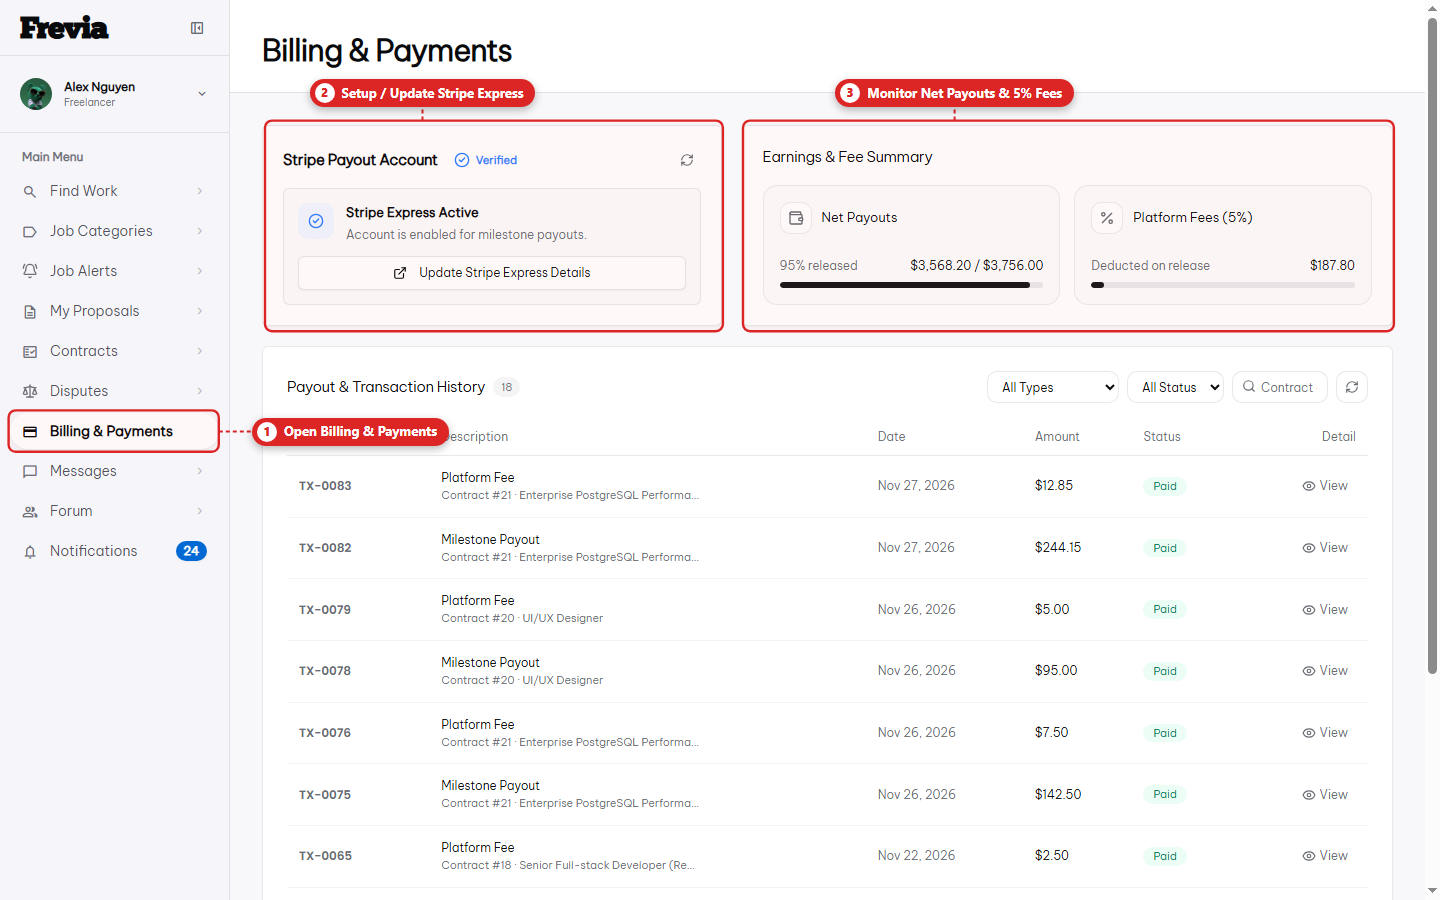
\includegraphics[width=0.90\textwidth]{images/payments/m43_01_connect_stripe_guide.png}
  \caption{Freelancer Billing \& Payments dashboard with Stripe Express onboarding card}
  \label{fig:m43_01_connect_stripe}
\end{figure}
\Needspace{6\baselineskip}\paragraph{Step-by-Step User Guide:}
\begin{enumerate}[leftmargin=1.8em,itemsep=3pt]
  \item \rbadge{1} \textbf{Open Billing \& Payments:} Select \textbf{Billing \& Payments} from the left navigation sidebar.
  \item \rbadge{2} \textbf{Setup / Update Stripe Express:} In the \textbf{Stripe Payout Account} panel, click \textbf{Connect with Stripe} (or \textbf{Update Stripe Express Details} if linked) to launch Stripe's secure Express onboarding form and provide bank/tax verification.
  \item \rbadge{3} \textbf{Monitor Net Payouts \& 5\% Fees:} Track cumulative net earnings (95\%) and deducted platform service fees (5\%) in \textbf{Earnings \& Fee Summary}.
\end{enumerate}
\Needspace{6\baselineskip}\paragraph{After You Submit (Result \& Troubleshooting):}
\begin{itemize}[leftmargin=1.5em,itemsep=2pt]
  \item \textbf{What Happens Next:} Upon completing Stripe Express onboarding and redirecting back to Frevia, your \texttt{stripeAccountId} activates automated milestone escrow disbursements.
  \item \textbf{Troubleshooting \& Common Messages:} Banking credentials stay exclusively within Stripe's PCI vault; never stored on Frevia servers.
\end{itemize}

% -----------------------------------------------------------------------------
\newpage
\subsubsection{M43.02 -- Check Stripe Connect Status (UC-43.02)}

\begin{itemize}[leftmargin=1.5em,itemsep=2pt]
  \item \textbf{Screen Name \& Route Path:} Stripe Payout Status Card -- \texttt{/freelancer/\allowbreak{}payments}.
  \item \textbf{Target Actor:} Freelancer.
  \item \Needspace{6\baselineskip}\textbf{Before You Begin:} Freelancer initiated Stripe Express onboarding.
\end{itemize}
\begin{figure}[H]\centering
  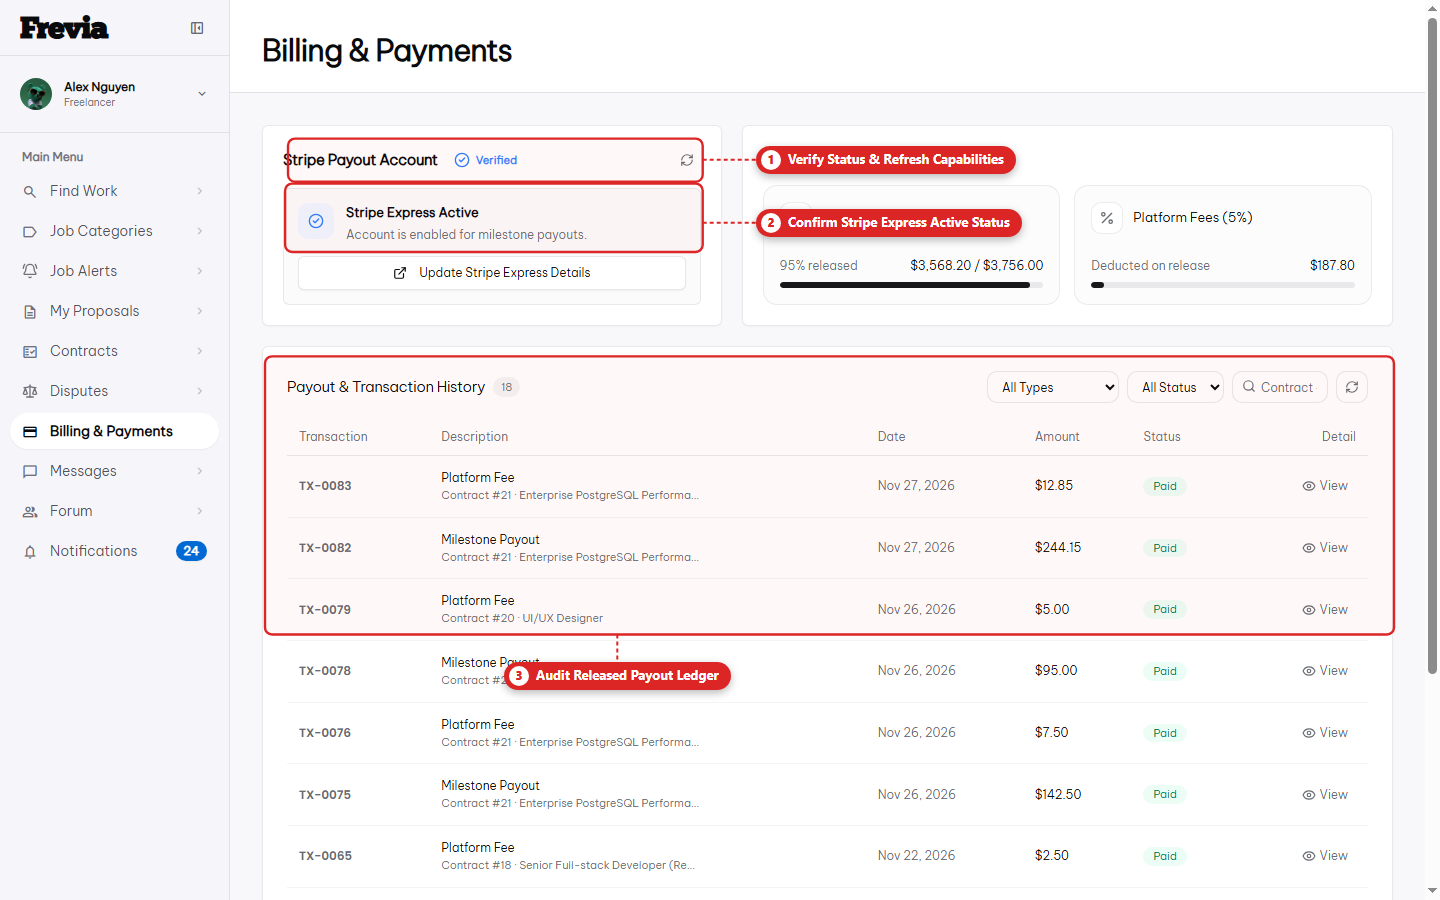
\includegraphics[width=0.90\textwidth]{images/payments/m43_02_check_stripe_status_guide.png}
  \caption{Verifying live Stripe Express readiness and payout capability status}
  \label{fig:m43_02_check_stripe_status}
\end{figure}
\Needspace{6\baselineskip}\paragraph{Step-by-Step User Guide:}
\begin{enumerate}[leftmargin=1.8em,itemsep=3pt]
  \item \rbadge{1} \textbf{Verify Status \& Refresh Capabilities:} Check the blue \textbf{Verified} badge beside \textit{Stripe Payout Account} and click the circular refresh icon to trigger \texttt{GET /api/payments/connect/status} if you just completed Stripe verification.
  \item \rbadge{2} \textbf{Confirm Stripe Express Active Status:} Ensure the status card reads \textit{``Stripe Express Active -- Account is enabled for milestone payouts''}.
  \item \rbadge{3} \textbf{Audit Released Payout Ledger:} Confirm incoming \textit{Milestone Payout} and \textit{Platform Fee} records show \textit{Paid} status below.
\end{enumerate}
\Needspace{6\baselineskip}\paragraph{After You Submit (Result \& Troubleshooting):}
\begin{itemize}[leftmargin=1.5em,itemsep=2pt]
  \item \textbf{What Happens Next:} Database readiness flags (\texttt{stripeOnboardingCompleted}) synchronize live with Stripe's \texttt{charges\_enabled} and \texttt{payouts\_enabled} states.
  \item \textbf{Troubleshooting \& Common Messages:} Accounts showing \textit{Action Required} or \textit{Restricted} require completing pending KYC prompts via \textbf{Update Stripe Express Details}.
\end{itemize}

% -----------------------------------------------------------------------------
\newpage
\subsubsection{M43.03 -- View Saved Payment Methods (UC-43.03)}

\begin{itemize}[leftmargin=1.5em,itemsep=2pt]
  \item \textbf{Screen Name \& Route Path:} Saved Payment Methods Modal -- \texttt{/client/\allowbreak{}payments}.
  \item \textbf{Target Actor:} Client.
  \item \Needspace{6\baselineskip}\textbf{Before You Begin:} Open \textbf{Billing \& Payments} as Client and click \textbf{Manage Cards}.
\end{itemize}
\begin{figure}[H]\centering
  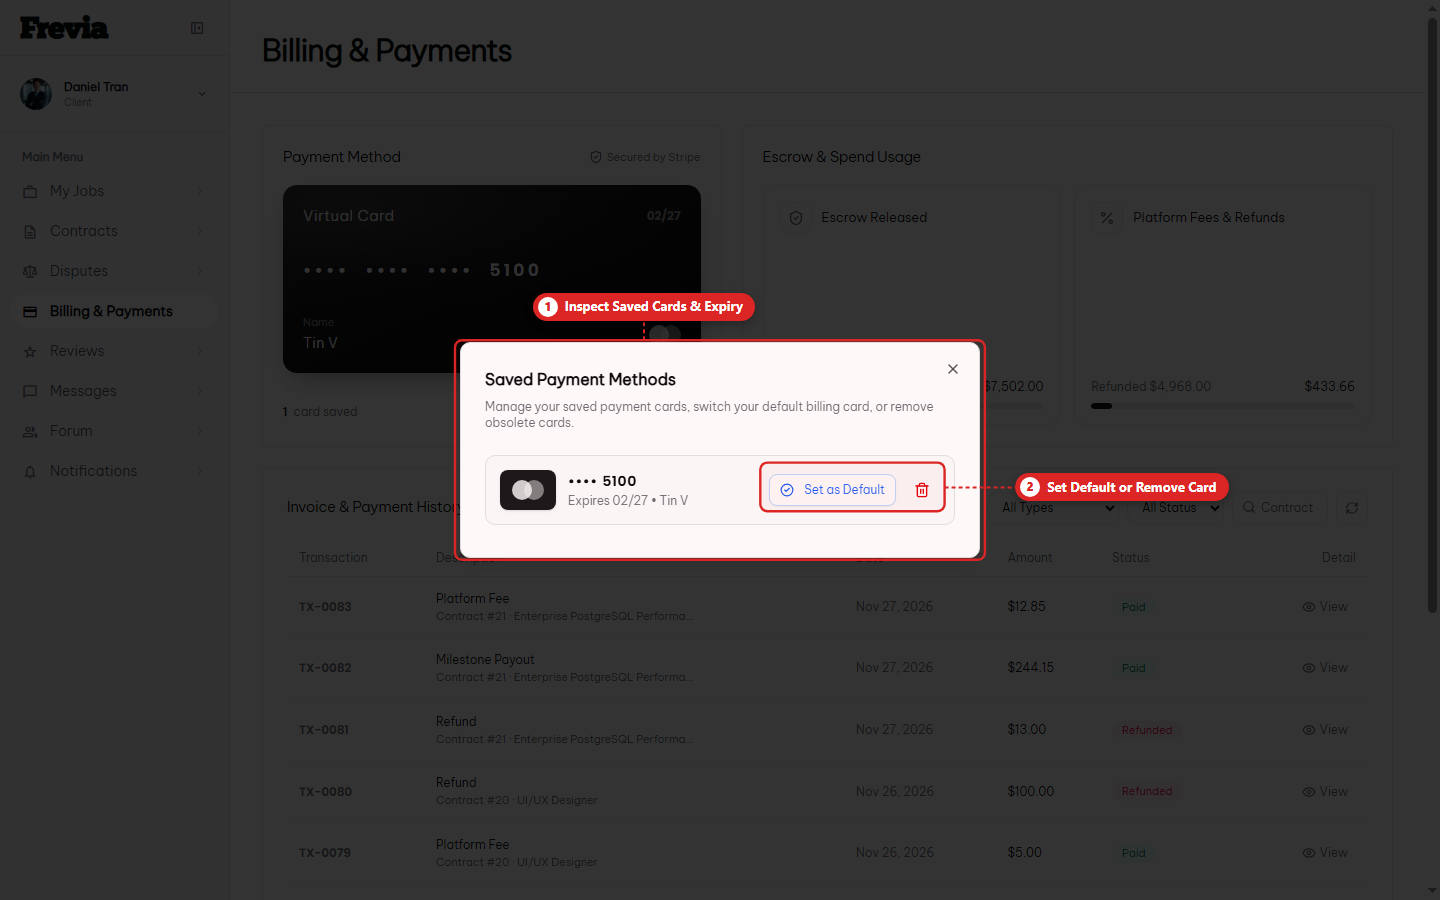
\includegraphics[width=0.90\textwidth]{images/payments/m43_03_view_payment_methods_guide.png}
  \caption{Saved Payment Methods wallet dialog displaying tokenized Stripe cards}
  \label{fig:m43_03_view_payment_methods}
\end{figure}
\Needspace{6\baselineskip}\paragraph{Step-by-Step User Guide:}
\begin{enumerate}[leftmargin=1.8em,itemsep=3pt]
  \item \rbadge{1} \textbf{Inspect Saved Cards \& Expiry:} Review card brand emblem (Mastercard/Visa), masked last 4 digits (e.g., \texttt{$\bullet\bullet\bullet\bullet$ 5100}), expiration date, and cardholder name.
  \item \rbadge{2} \textbf{Set Default or Remove Card:} Use the per-card controls to promote a card as default or delete expired cards.
\end{enumerate}
\Needspace{6\baselineskip}\paragraph{After You Submit (Result \& Troubleshooting):}
\begin{itemize}[leftmargin=1.5em,itemsep=2pt]
  \item \textbf{What Happens Next:} Tokenized cards attached to your Stripe Customer profile appear securely without exposing full PAN/CVV numbers.
  \item \textbf{Troubleshooting \& Common Messages:} Cards saved during prior Stripe Checkout sessions automatically populate in this wallet.
\end{itemize}

% -----------------------------------------------------------------------------
\newpage
\subsubsection{M43.04 -- Set Default Payment Method (UC-43.04)}

\begin{itemize}[leftmargin=1.5em,itemsep=2pt]
  \item \textbf{Screen Name \& Route Path:} Saved Payment Methods Modal -- \texttt{/client/\allowbreak{}payments}.
  \item \textbf{Target Actor:} Client.
  \item \Needspace{6\baselineskip}\textbf{Before You Begin:} At least one non-default saved payment card exists in your Stripe Customer wallet.
\end{itemize}
\begin{figure}[H]\centering
  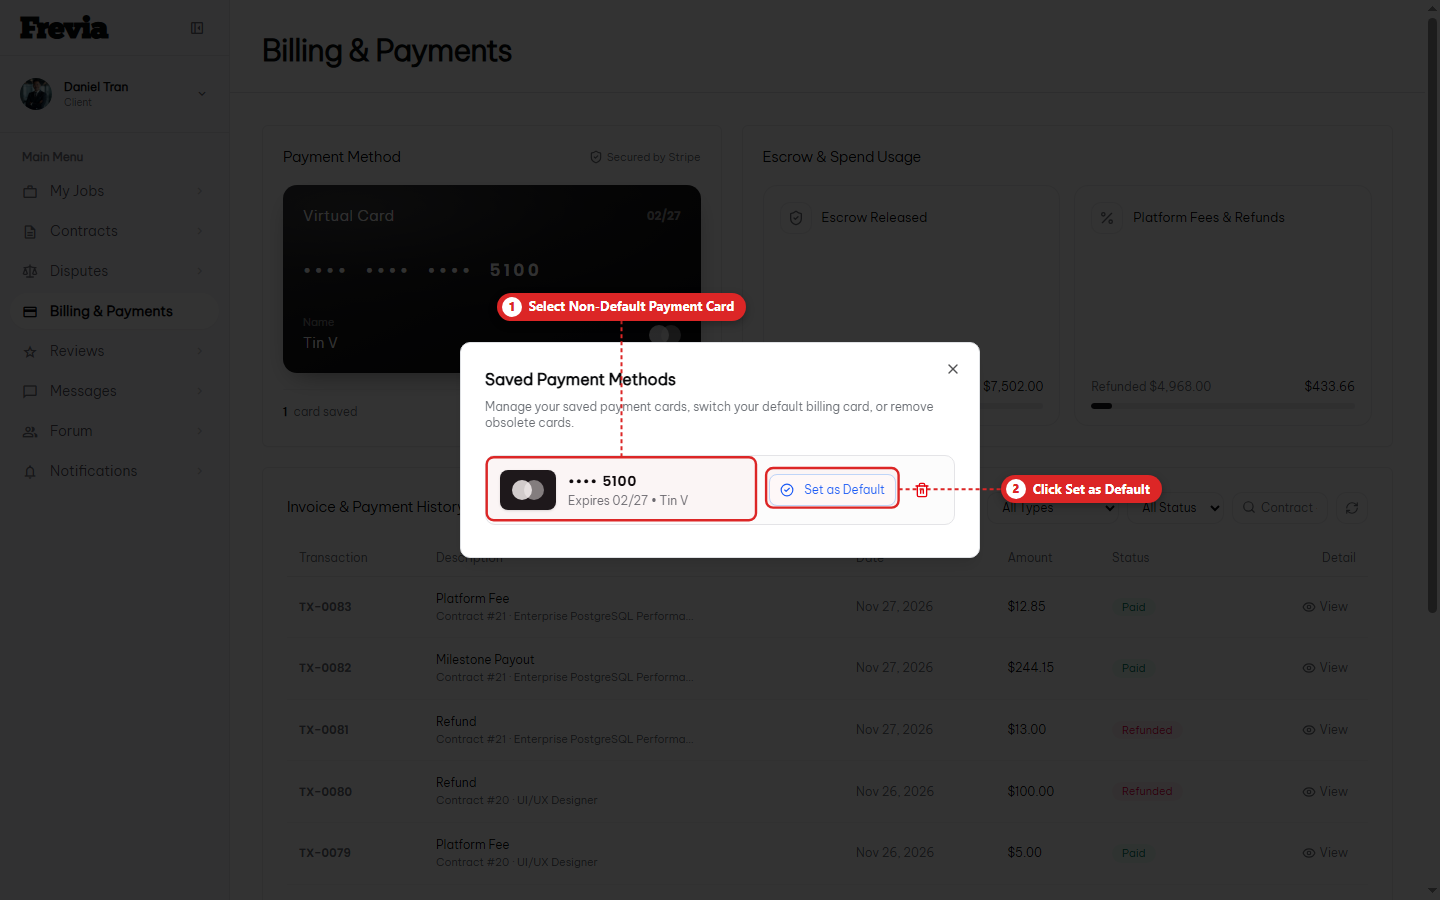
\includegraphics[width=0.90\textwidth]{images/payments/m43_04_set_default_payment_method_guide.png}
  \caption{Promoting a saved Stripe card as the default funding method}
  \label{fig:m43_04_set_default_payment_method}
\end{figure}
\Needspace{6\baselineskip}\paragraph{Step-by-Step User Guide:}
\begin{enumerate}[leftmargin=1.8em,itemsep=3pt]
  \item \rbadge{1} \textbf{Select Non-Default Payment Card:} Locate the card row without the \textit{Default} badge inside the \textbf{Saved Payment Methods} dialog.
  \item \rbadge{2} \textbf{Click Set as Default:} Click \textbf{Set as Default} next to the card to assign it as your Stripe Customer's default invoice/payment source.
\end{enumerate}
\Needspace{6\baselineskip}\paragraph{After You Submit (Result \& Troubleshooting):}
\begin{itemize}[leftmargin=1.5em,itemsep=2pt]
  \item \textbf{What Happens Next:} The selected card updates on the primary Billing Virtual Card display and pre-selects automatically during future 1-click escrow deposits.
  \item \textbf{Troubleshooting \& Common Messages:} Cards belonging to another Stripe customer account cannot be set as default.
\end{itemize}

% -----------------------------------------------------------------------------
\newpage
\subsubsection{M43.05 -- Remove Saved Payment Method (UC-43.05)}

\begin{itemize}[leftmargin=1.5em,itemsep=2pt]
  \item \textbf{Screen Name \& Route Path:} Remove Payment Method Modal -- \texttt{/client/\allowbreak{}payments}.
  \item \textbf{Target Actor:} Client.
  \item \Needspace{6\baselineskip}\textbf{Before You Begin:} Click the red trash icon beside a card in \textbf{Saved Payment Methods}.
\end{itemize}
\begin{figure}[H]\centering
  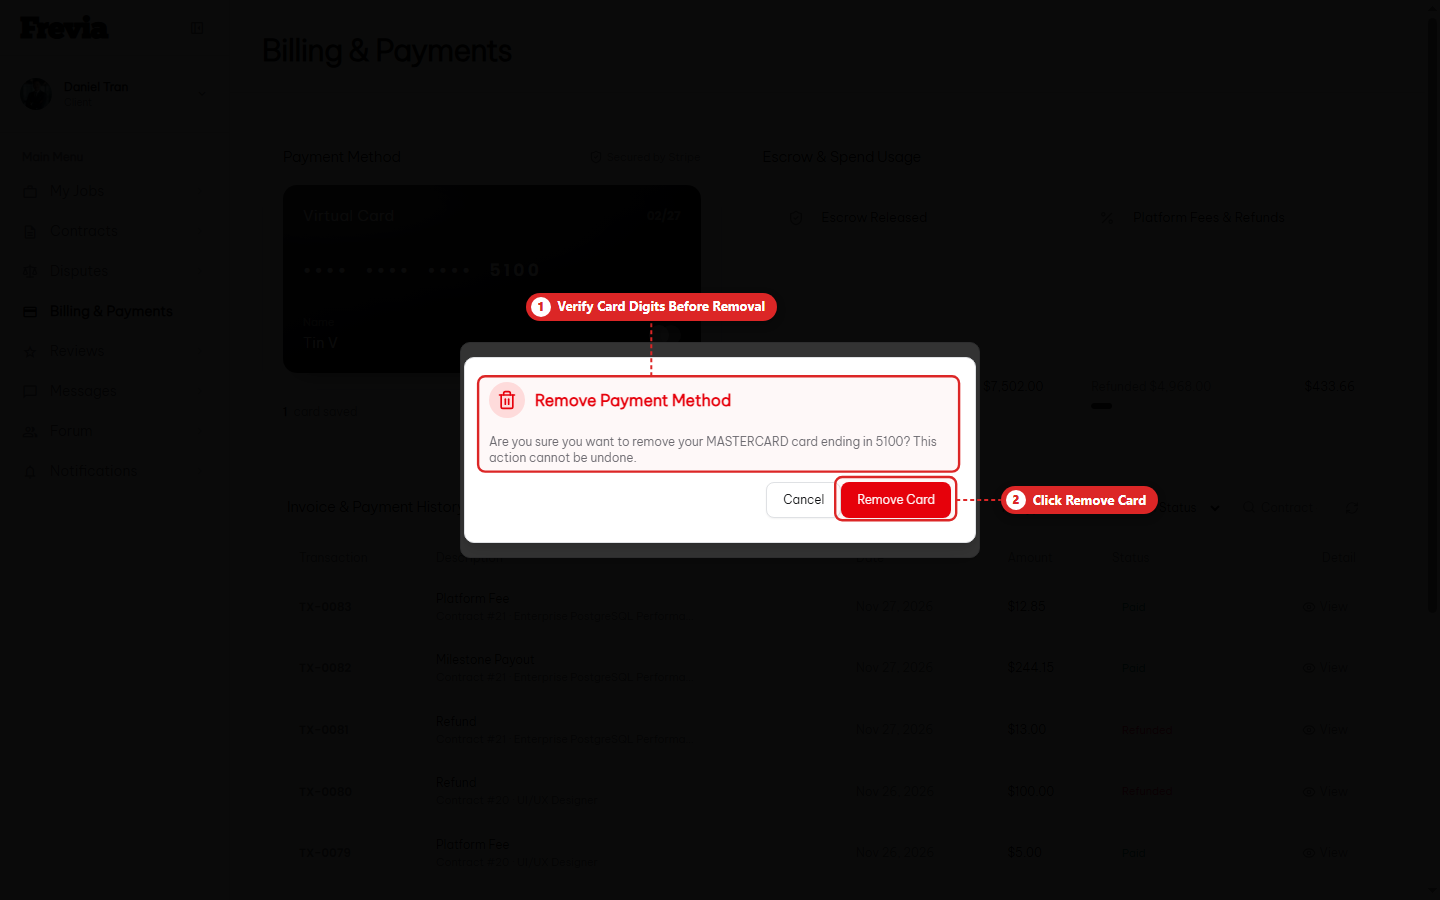
\includegraphics[width=0.90\textwidth]{images/payments/m43_05_remove_payment_method_guide.png}
  \caption{Remove Payment Method confirmation dialog showing masked last 4 digits}
  \label{fig:m43_05_remove_payment_method}
\end{figure}
\Needspace{6\baselineskip}\paragraph{Step-by-Step User Guide:}
\begin{enumerate}[leftmargin=1.8em,itemsep=3pt]
  \item \rbadge{1} \textbf{Verify Card Digits Before Removal:} Check the card brand and trailing 4 digits in the confirmation warning.
  \item \rbadge{2} \textbf{Click Remove Card:} Click the red \textbf{Remove Card} button to detach the payment method from Stripe immediately.
\end{enumerate}
\Needspace{6\baselineskip}\paragraph{After You Submit (Result \& Troubleshooting):}
\begin{itemize}[leftmargin=1.5em,itemsep=2pt]
  \item \textbf{What Happens Next:} The card detaches cleanly in Stripe and disappears from your saved wallet count.
  \item \textbf{Troubleshooting \& Common Messages:} Already-authorized contract holds or active escrows remain unaffected by detaching a card afterwards.
\end{itemize}

% -----------------------------------------------------------------------------
\newpage
\subsubsection[M43.06 -- Create Contract Hold Deposit (UC-43.06)]{M43.06 -- Authorize Contract Escrow Hold (UC-43.06)}

\begin{itemize}[leftmargin=1.5em,itemsep=2pt]
  \item \textbf{Screen Name \& Route Path:} Authorize Contract Escrow Hold Drawer -- \texttt{/client/\allowbreak{}contracts/\allowbreak{}[slug]}.
  \item \textbf{Target Actor:} Client.
  \item \Needspace{6\baselineskip}\textbf{Before You Begin:} Contract is in \texttt{AWAITING\_PAYMENT} status and requires pre-signing hold authorization.
\end{itemize}
\begin{figure}[H]\centering
  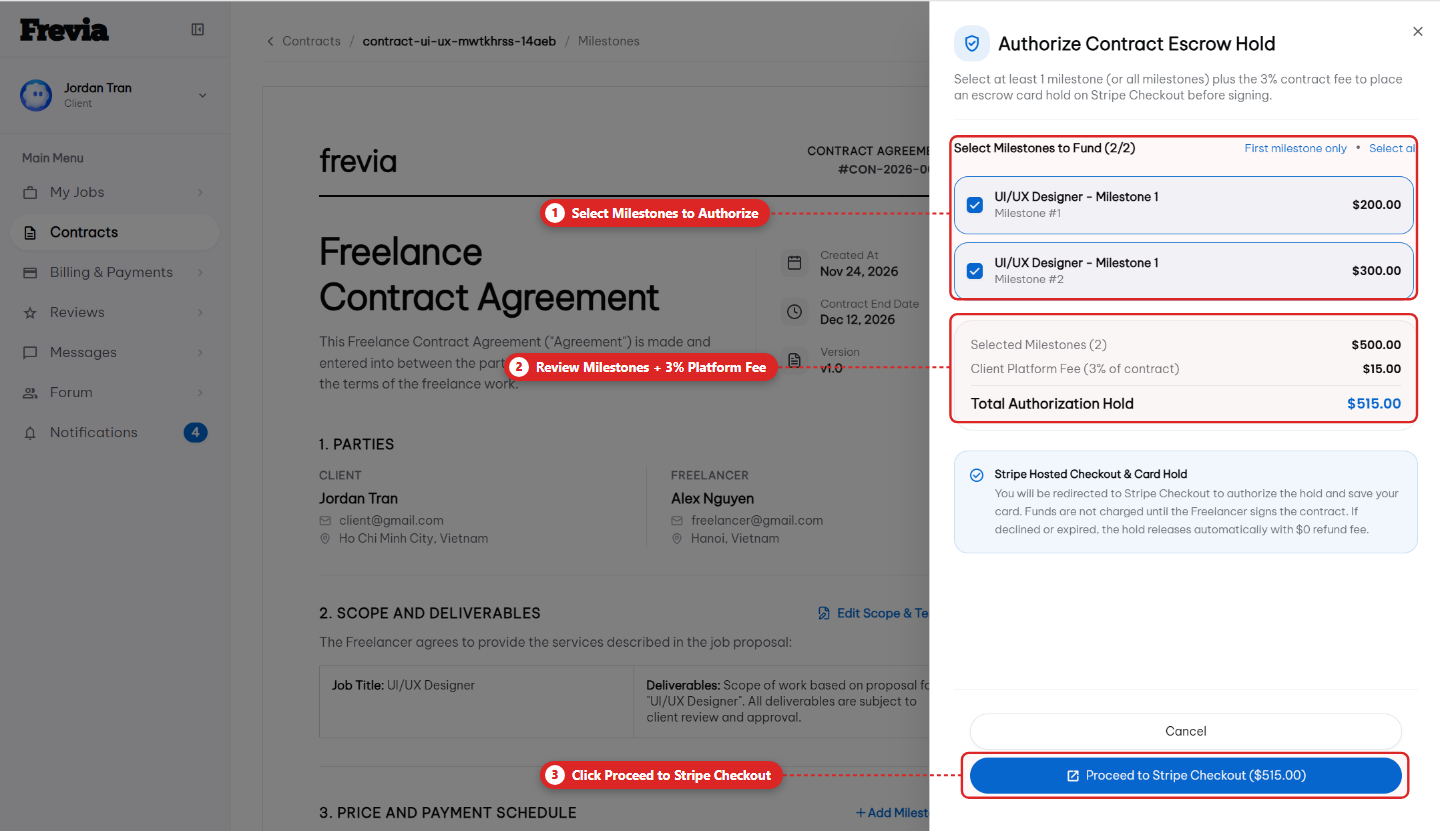
\includegraphics[width=0.90\textwidth]{images/payments/m43_06_contract_hold_deposit_guide.png}
  \caption{Authorize Contract Escrow Hold drawer calculating selected milestones plus 3\% client fee}
  \label{fig:m43_06_contract_hold_deposit}
\end{figure}
\Needspace{6\baselineskip}\paragraph{Step-by-Step User Guide:}
\begin{enumerate}[leftmargin=1.8em,itemsep=3pt]
  \item \rbadge{1} \textbf{Select Milestones to Authorize:} Tick at least one milestone (or click \textbf{Select all} / \textbf{First milestone only}) to fund alongside signing.
  \item \rbadge{2} \textbf{Review Milestones + 3\% Platform Fee:} Verify the subtotal of selected milestones, the 3\% Client Platform Fee, and \textit{Total Authorization Hold}.
  \item \rbadge{3} \textbf{Click Proceed to Stripe Checkout:} Click the blue \textbf{Proceed to Stripe Checkout} button to place a card authorization hold (captured only once the Freelancer countersigns).
\end{enumerate}
\Needspace{6\baselineskip}\paragraph{After You Submit (Result \& Troubleshooting):}
\begin{itemize}[leftmargin=1.5em,itemsep=2pt]
  \item \textbf{What Happens Next:} Upon Checkout/Intent completion and automatic PaymentIntent sync (\texttt{UC-43.11}), the contract transitions to \texttt{PENDING\_SIGN}. If the Freelancer declines or the contract expires, the hold auto-releases with \$0 refund fee.
  \item \textbf{Troubleshooting \& Common Messages:} At least one milestone must remain selected before Checkout initiation is permitted.
\end{itemize}

% -----------------------------------------------------------------------------
\newpage
\subsubsection{M43.07 -- Fund Milestone via Stripe Checkout (UC-43.07)}

\begin{itemize}[leftmargin=1.5em,itemsep=2pt]
  \item \textbf{Screen Name \& Route Path:} Hosted Stripe Checkout Portal -- \texttt{checkout.stripe.com}.
  \item \textbf{Target Actor:} Client.
  \item \Needspace{6\baselineskip}\textbf{Before You Begin:} Click \textbf{Fund Escrow} $\rightarrow$ \textbf{Deposit via Stripe} on an unfunded active milestone.
\end{itemize}
\begin{figure}[H]\centering
  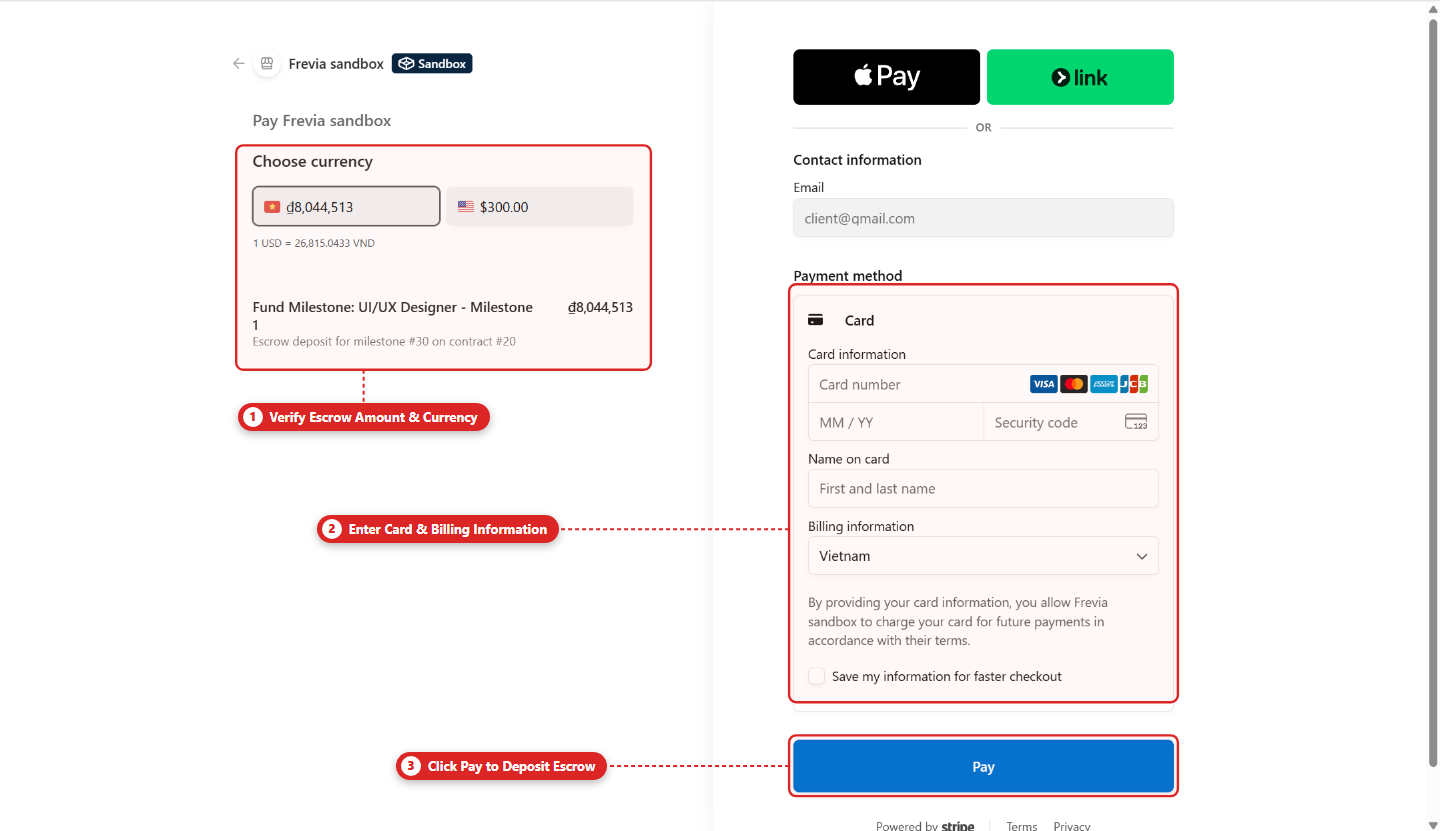
\includegraphics[width=0.90\textwidth]{images/payments/m43_07_fund_milestone_checkout_guide.png}
  \caption{Hosted Stripe Checkout page for milestone escrow deposit}
  \label{fig:m43_07_fund_milestone_checkout}
\end{figure}
\Needspace{6\baselineskip}\paragraph{Step-by-Step User Guide:}
\begin{enumerate}[leftmargin=1.8em,itemsep=3pt]
  \item \rbadge{1} \textbf{Verify Escrow Amount \& Currency:} Check the milestone description, escrow deposit amount, and currency toggle on the left summary panel.
  \item \rbadge{2} \textbf{Enter Card \& Billing Information:} Provide card number, expiry (\textit{MM/YY}), CVC, cardholder name, and country; optionally tick \textit{Save my information} or complete 3D Secure.
  \item \rbadge{3} \textbf{Click Pay to Deposit Escrow:} Click \textbf{Pay} to complete payment and redirect back to Frevia.
\end{enumerate}
\Needspace{6\baselineskip}\paragraph{After You Submit (Result \& Troubleshooting):}
\begin{itemize}[leftmargin=1.5em,itemsep=2pt]
  \item \textbf{What Happens Next:} Both return-URL Checkout Session Sync (\texttt{UC-43.12}) and Stripe Webhook verification (\texttt{UC-43.13}) reconcile payment state immediately, transitioning the milestone to \texttt{FUNDED} (\textit{Escrow Funded}).
  \item \textbf{Troubleshooting \& Common Messages:} In sandbox testing, use Stripe test cards (e.g., \texttt{4242~4242...}); declined cards stay on Checkout for retry without altering escrow balances.
\end{itemize}

% -----------------------------------------------------------------------------
\newpage
\subsubsection{M43.08 -- Fund Milestone with Saved Card (UC-43.08)}

\begin{itemize}[leftmargin=1.5em,itemsep=2pt]
  \item \textbf{Screen Name \& Route Path:} Fund Milestone Escrow Drawer -- \texttt{/client/\allowbreak{}contracts/\allowbreak{}[slug]/\allowbreak{}milestones}.
  \item \textbf{Target Actor:} Client.
  \item \Needspace{6\baselineskip}\textbf{Before You Begin:} Contract is \texttt{ACTIVE} and target milestone is in \texttt{Pending Escrow} state (click \textbf{Fund Escrow}).
\end{itemize}
\begin{figure}[H]\centering
  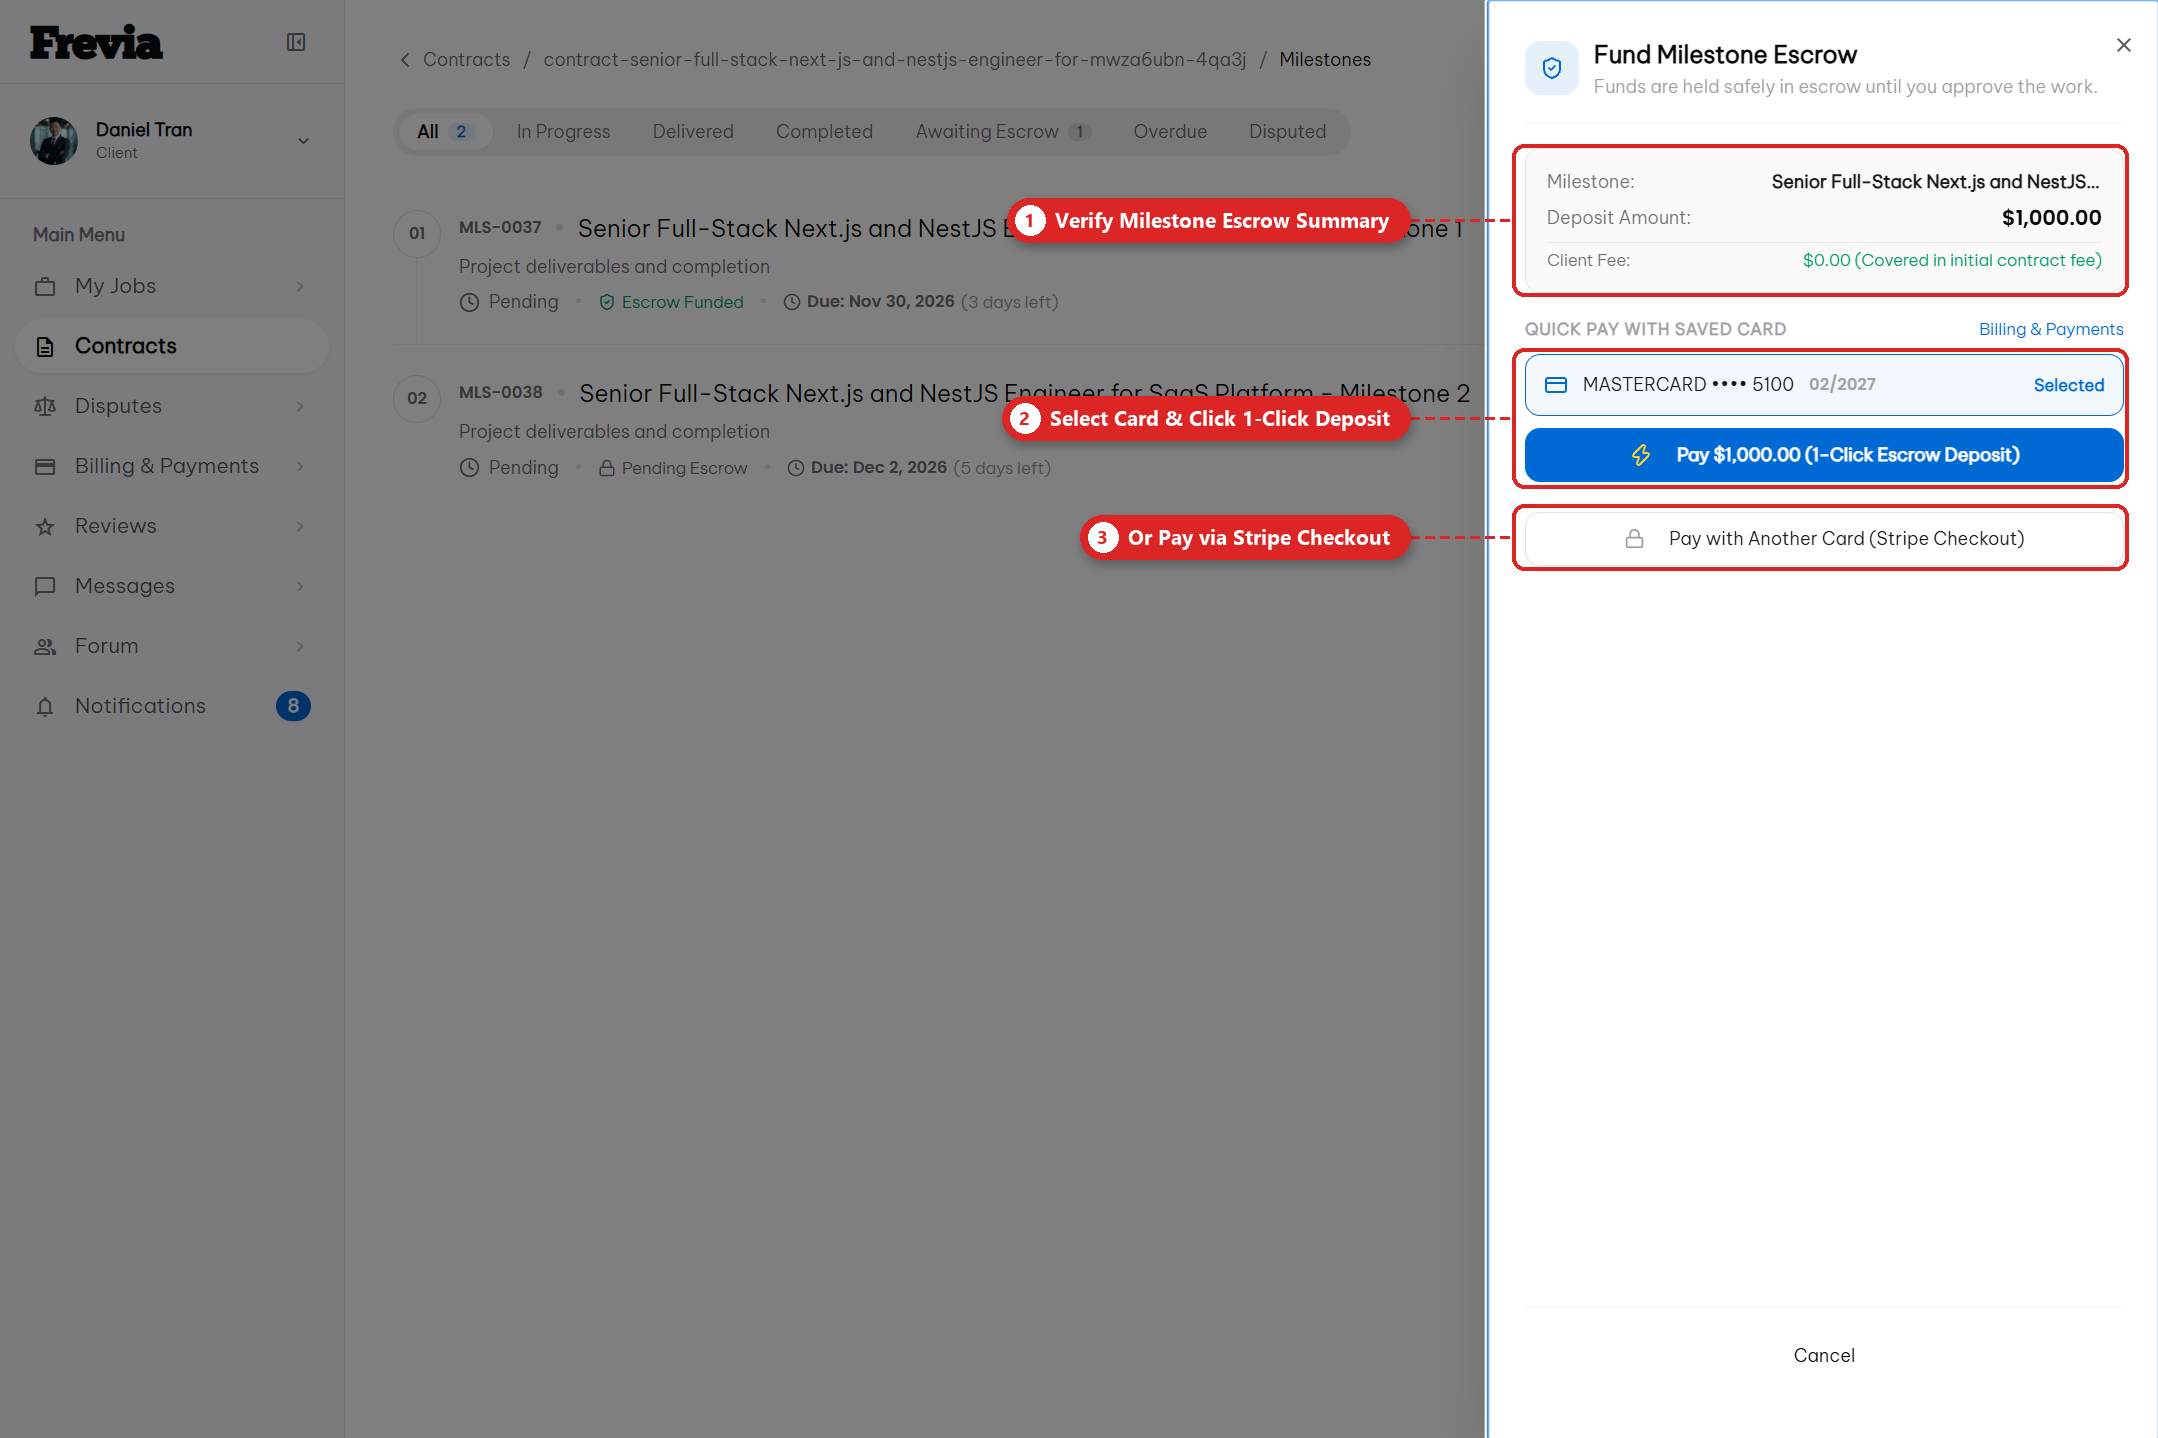
\includegraphics[width=0.90\textwidth]{images/payments/m43_08_fund_milestone_saved_card_guide.png}
  \caption{Fund Milestone Escrow drawer with 1-Click Saved Card deposit and fallback Stripe Checkout option}
  \label{fig:m43_08_fund_milestone_saved_card}
\end{figure}
\Needspace{6\baselineskip}\paragraph{Step-by-Step User Guide:}
\begin{enumerate}[leftmargin=1.8em,itemsep=3pt]
  \item \rbadge{1} \textbf{Verify Milestone Escrow Summary:} Review the milestone name, exact \textit{Deposit Amount}, and confirmation that \textit{Client Fee} is \texttt{\$0.00 (Covered in initial contract fee)}.
  \item \rbadge{2} \textbf{Select Card \& Click 1-Click Deposit:} Confirm your saved card under \textit{QUICK PAY WITH SAVED CARD} and click \textbf{Pay \$X.00 (1-Click Escrow Deposit)} (then confirm in the modal) for instant off-session charging.
  \item \rbadge{3} \textbf{Or Pay via Stripe Checkout:} Click \textbf{Pay with Another Card (Stripe Checkout)} to redirect to Stripe Checkout instead, or \textbf{Cancel} to exit without charging.
\end{enumerate}
\Needspace{6\baselineskip}\paragraph{After You Submit (Result \& Troubleshooting):}
\begin{itemize}[leftmargin=1.5em,itemsep=2pt]
  \item \textbf{What Happens Next:} Funds lock safely inside platform Escrow, unlocking \textbf{Start Work} for the Freelancer and recording a \textit{DEPOSIT} ledger entry.
  \item \textbf{Troubleshooting \& Common Messages:} If 3D Secure authentication is required by the card issuer, PaymentIntent Sync (\texttt{UC-43.11}) reconciles completion immediately upon modal dismissal.
\end{itemize}

% -----------------------------------------------------------------------------
\newpage
\subsubsection[M43.09 -- Release Milestone Escrow (UC-43.09)]{M43.09 -- Release Milestone Escrow Payment (UC-43.09)}

\begin{itemize}[leftmargin=1.5em,itemsep=2pt]
  \item \textbf{Screen Name \& Route Path:} Review Work Submission Drawer -- \texttt{/client/\allowbreak{}contracts/\allowbreak{}[slug]/\allowbreak{}milestones/\allowbreak{}[milestoneId]}.
  \item \textbf{Target Actor:} Client.
  \item \Needspace{6\baselineskip}\textbf{Before You Begin:} Freelancer has delivered milestone work (\texttt{SUBMITTED}) and the milestone holds \texttt{FUNDED} escrow.
\end{itemize}
\begin{figure}[H]\centering
  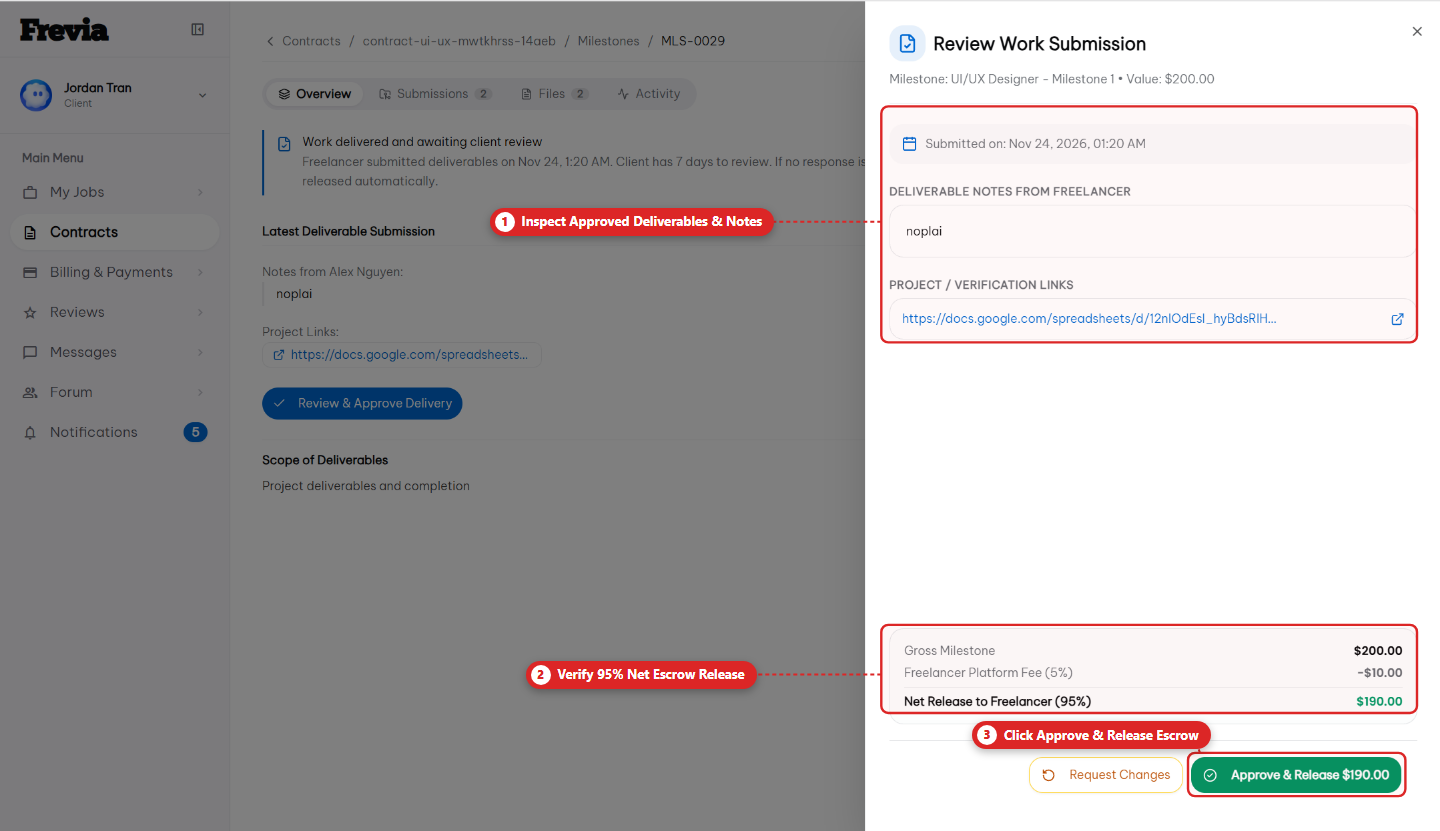
\includegraphics[width=0.90\textwidth]{images/payments/m43_09_release_milestone_escrow_guide.png}
  \caption{Releasing 95\% milestone escrow funds to Freelancer via Stripe Connect}
  \label{fig:m43_09_release_milestone_escrow}
\end{figure}
\Needspace{6\baselineskip}\paragraph{Step-by-Step User Guide:}
\begin{enumerate}[leftmargin=1.8em,itemsep=3pt]
  \item \rbadge{1} \textbf{Inspect Approved Deliverables \& Notes:} Verify submitted notes, attachments, and preview links fulfill deliverable expectations.
  \item \rbadge{2} \textbf{Verify 95\% Net Escrow Release:} Confirm gross milestone budget, 5\% Freelancer platform fee, and final net payout transfer amount.
  \item \rbadge{3} \textbf{Click Approve \& Release Escrow:} Click the green \textbf{Approve \& Release} button to finalize approval and execute the Stripe Connect transfer.
\end{enumerate}
\Needspace{6\baselineskip}\paragraph{After You Submit (Result \& Troubleshooting):}
\begin{itemize}[leftmargin=1.5em,itemsep=2pt]
  \item \textbf{What Happens Next:} Milestone payment status updates to \textit{Released}, Stripe disburses 95\% net funds to the Freelancer's connected account, and both \textit{Milestone Payout} and \textit{Platform Fee} ledger rows finalize.
  \item \textbf{Troubleshooting \& Common Messages:} Milestones currently under active dispute cannot be manually released until arbitration concludes.
\end{itemize}

% -----------------------------------------------------------------------------
\newpage
\subsubsection[M43.10 -- Payment History & Sync (UC-43.10--43.13)]{M43.10 -- View Payment Transactions History \& Automated Sync (UC-43.10 to UC-43.13)}

\begin{itemize}[leftmargin=1.5em,itemsep=2pt]
  \item \textbf{Screen Name \& Route Path:} Billing \& Payments Ledger -- \texttt{/client/\allowbreak{}payments} or \texttt{/freelancer/\allowbreak{}payments}.
  \item \textbf{Target Actor:} Client, Freelancer.
  \item \Needspace{6\baselineskip}\textbf{Before You Begin:} Signed in with an active Client or Freelancer account.
\end{itemize}
\begin{figure}[H]\centering
  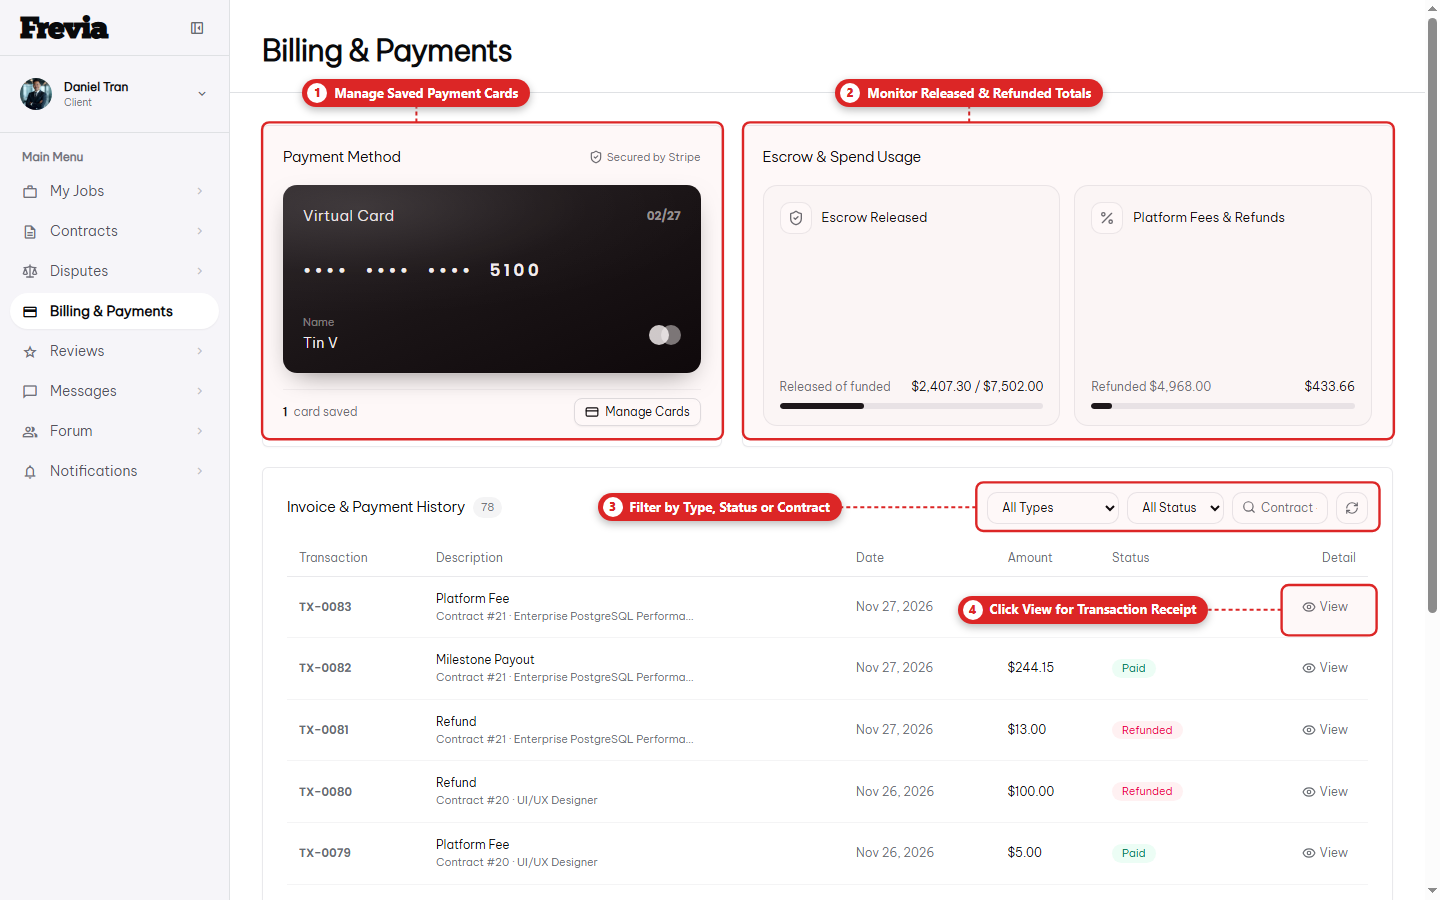
\includegraphics[width=0.90\textwidth]{images/payments/m43_10_view_payment_transactions_guide.png}
  \caption{Billing \& Payments ledger with saved card preview, escrow spend metrics, and filters}
  \label{fig:m43_10_view_payment_transactions}
\end{figure}
\Needspace{6\baselineskip}\paragraph{Step-by-Step User Guide:}
\begin{enumerate}[leftmargin=1.8em,itemsep=3pt]
  \item \rbadge{1} \textbf{Manage Saved Payment Cards:} Review your default card summary or click \textbf{Manage Cards} to add, switch default, or remove cards.
  \item \rbadge{2} \textbf{Monitor Released \& Refunded Totals:} Track cumulative Escrow Released, total funded volume, platform fees, and arbitration refunds.
  \item \rbadge{3} \textbf{Filter by Type, Status or Contract:} Use \textit{All Types}, \textit{All Status}, or the contract search box to isolate deposits, payouts, fees, or refunds.
  \item \rbadge{4} \textbf{Click View for Transaction Receipt:} Click \textbf{View} beside any row (e.g., \texttt{TX-0083}) to open the detailed transaction receipt drawer.
\end{enumerate}
\Needspace{6\baselineskip}\paragraph{After You Submit (Result \& Troubleshooting):}
\begin{itemize}[leftmargin=1.5em,itemsep=2pt]
  \item \textbf{What Happens Next:} All ledger movements synchronize reliably via three automated backend safeguards: \textbf{Sync Payment Intent Status (\texttt{UC-43.11})} after 3DS verification, \textbf{Sync Checkout Session Status (\texttt{UC-43.12})} on Stripe return redirects, and \textbf{Stripe Webhook Events (\texttt{UC-43.13})} verifying \texttt{stripe-signature} HMAC SHA-256 events server-to-server.
  \item \textbf{Troubleshooting \& Common Messages:} If a payment appears briefly pending immediately after returning from Stripe Checkout, wait a few seconds or reload the Billing/Contract view to trigger fallback session reconciliation automatically.
\end{itemize}
